\documentclass[10pt]{article}

\usepackage[margin=0.75in]{geometry}
\usepackage{amsmath,amsthm,amssymb,bm}
\usepackage{xcolor}
\usepackage{cancel}
\usepackage{graphicx}
\usepackage{changepage}
\usepackage{circuitikz}
\usepackage{pgfplots}
\usepackage{minted}
\usepackage{physics}
\usepackage{tikz}
\usepackage{tikz-3dplot}
\usepackage{hyperref}
\usepackage{siunitx}
\usepackage{fontspec}
\usepackage{relsize}
\usepackage{subfig}
\usepackage{todonotes}
\usepackage{contour}
\usepackage{multicol, multirow, booktabs}
\usepackage[breakable]{tcolorbox}
\usepackage[inline]{enumitem}

\theoremstyle{definition}
\newtheorem{problem}{Problem}
\newtheorem{soln}{Solution}

\pgfplotsset{compat=newest}
\usetikzlibrary{lindenmayersystems}
\usetikzlibrary{arrows}
\usetikzlibrary{calc}
\usetikzlibrary{positioning, fit}
\usetikzlibrary{3d, perspective}
\usetikzlibrary{math}
\usetikzlibrary{fadings}
\usetikzlibrary{angles,quotes} 
\usetikzlibrary{decorations.markings}
\usetikzlibrary{tikzmark}

\definecolor{incolor}{HTML}{303F9F}
\definecolor{outcolor}{HTML}{D84315}
\definecolor{cellborder}{HTML}{CFCFCF}
\definecolor{cellbackground}{HTML}{F7F7F7}
\newcommand{\ui}{\hat{i}}
\newcommand{\uj}{\hat{j}}
\newcommand{\uk}{\hat{k}}
\newcommand{\ux}{\hat{\mathbf{x}}}
\newcommand{\uy}{\hat{\mathbf{y}}}
\newcommand{\uz}{\hat{\mathbf{z}}}
\newcommand{\uv}[1]{\hat{\bv{{#1}}}}
\newcommand{\pr}[1]{{#1^\prime}}
\newcommand{\pd}[2][]{{\frac{\partial^{#1}}{\partial {{#2}^{#1}}}}}
\newcommand{\dif}[2][]{{\frac{d^{#1}}{d{{#2}^{#1}}}}}
\newcommand{\grd}{\nabla}

\pgfdeclarelayer{background}  
\pgfsetlayers{background,main}
\AtBeginDocument{\RenewCommandCopy\qty\SI}

\makeatletter
\newcommand{\boxspacing}{\kern\kvtcb@left@rule\kern\kvtcb@boxsep}
\makeatother
\newcommand{\prompt}[4]{
    \ttfamily\llap{{\color{#2}[#3]:\hspace{3pt}#4}}\vspace{-\baselineskip}
}

\newcommand{\thevenin}[2]{
  \begin{center}
    \begin{circuitikz} \draw
      (0,0) -- (2,0) to[battery1, l_=$V_{Th}\eq#1$] (2,2) 
      to[resistor, l_=$R_{Th}\eq#2$] (0,2)
      ;
      \draw [o-] (-.07,2.079);
      \draw [o-] (-.07,0.079);
    \end{circuitikz}
  \end{center}
}

\newcommand{\norton}[2]{
  \begin{center}
    \begin{circuitikz} \draw
      (0,0) -- (3,0) to[american current source, l_=$I_{N}\eq#1$] (3,2) -- (0,2) (2,0)
      to[resistor, l=$R_{N}\eq#2$] (2,2)
      ;
      \draw [o-] (-.07,2.079);
      \draw [o-] (-.07,0.079);
    \end{circuitikz}
  \end{center}
}

\DeclareMathOperator{\Div}{div}
\DeclareMathOperator{\Curl}{curl}
\DeclareMathOperator{\sgn}{sgn}
\DeclareMathOperator{\erfc}{erfc}

\newcommand{\highlight}[1]{\colorbox{yellow}{$\displaystyle #1$}}
\newcommand{\ti}[1]{\widetilde{#1}}
\renewcommand{\div}[1]{\bv{\nabla}\cdot #1}
\renewcommand{\curl}[1]{\bv{\nabla}\times #1}

\newfontface{\Kaufmann}{Kaufmann}
\DeclareTextFontCommand{\kf}{\Kaufmann}
\newcommand{\scriptr}{\fontsize{12pt}{12pt}\kf{r}\fontsize{10pt}{10pt}}

\newfontface{\KaufmannB}{Kaufmann Bold}
\DeclareTextFontCommand{\kfb}{\KaufmannB}
\newcommand{\bscriptr}{\fontsize{12pt}{12pt}\kfb{r}\fontsize{10pt}{10pt}}
\newcommand{\justif}[2]{&{#1}&\text{#2}}
\newcommand{\bv}[1]{\bm{\mathrm{#1}}}

\title{Physics 4700H: Assignment VI}
\author{Jeremy Favro (0805980) \\ Trent University, Peterborough, ON, Canada}
\date{\today}

\begin{document}
\maketitle

% PROBLEM 1
\begin{problem} Consider a system which can be in one of three states, corresponding to energies $\xi_1$, $\xi_2$,
and $\xi_3$. What is the partition function of this system?
\end{problem}
\begin{soln}
  $$Z=\sum_ip_i=\sum_ie^{\xi_i/k_BT}=e^{\xi_1/k_BT}+e^{\xi_2/k_BT}+e^{\xi_3/k_BT}.$$
\end{soln}

% PROBLEM 2
\begin{problem}
In class we found that for a two state system $F = -k_BT\ln(1+e^{-\epsilon/k_BT})$. What is the
entropy of this system as a function of temperature? Consider the value of your result at
$T = 0$ and $T \to \infty $. Comment on whether the values you get make sense.
\end{problem}
\begin{soln}
  Recall that $dF=dU-TdS-SdT$. In the microcanonical ensemble (reservoir plus system),
  $$\left.-\frac{\partial F}{\partial T}\right)_{N,V,U,S}=S.$$
  Then we just differentiate the expression we have for $F$,
  $$S=
    k_B\ln(1+e^{-\epsilon/k_BT})+\frac{k_BT}{1+e^{-\epsilon/k_BT}}\left[\frac{\epsilon}{k_BT^2}e^{-\epsilon/k_BT}\right]
    =k_B\ln(1+e^{-\epsilon/k_BT})+\frac{\epsilon e^{-\epsilon/k_BT}}{\left[1+e^{-\epsilon/k_BT}\right]T}.
  $$
  In the $T=0$ case, $e^{-\epsilon/k_BT}\to e^{-\infty}\to 0$, so the first term goes to zero as $\ln(1)=0$. The second term's
  numerator goes to zero, as does the denominator, but the denominator is bounded by
  $$T\leq \left[1+e^{-\epsilon/k_BT}\right]T,$$
  so the entire fraction is bounded by
  $$\frac{\epsilon e^{-\epsilon/k_BT}}{\left[1+e^{-\epsilon/k_BT}\right]T}\leq \frac{\epsilon e^{-\epsilon/k_BT}}{T}$$
  (reciprocal flips the inequality, if you want)
  which certainly goes to zero as exponentials beat polynomials. Then since the original expression is less than something going to zero but is itself
  greater than zero, $S(0)\to 0$.


  In the $S(T\to\infty)$ case, $e^{-\epsilon/k_BT}\to e^{0}\to 1$ so the first term goes to $k_B\ln(2)$ and the second goes like $1/T$, which goes to zero at large $T$,
  hence $S(T\to\infty)=k_B\ln(2)$. The first value certainly makes sense, it is a law of thermodynamics that $S(0)\to 0$ in most systems.
  The second result is consistent with the Gibbs entropy provided the two states are equally likely,
  $$S_G=-k_B\sum_ip_i\ln p_i=k_B\left[\frac{\ln(2)}{2}+\frac{\ln(2)}{2}\right]$$
  where I pulled the negative into the $\ln$ to flip the probability, and took $p_i=1/2$. I'm not totally sure this is the correct understanding of
  what's happening but it works.
\end{soln}
\newpage

% PROBLEM 3
\begin{problem}
Replacing sums by integrals
\begin{enumerate}[label=(\alph*)]
  \item Show that $\sum_{n=0}^{\infty}u^n=1/(1-u)$ for $u<1$.
  \item Consider the function $f (n) = e^{-Cn}$ where $n$ is a non-negative integer. Make a sketch
        showing $f (n)$ for $C = 0.1$, $1$ and $10$.
  \item Calculate and compare
        $$S_{10}=\sum_{n=1}^{\infty}e^{-10n}\quad \text{and}\quad I_{10}=\int_0^\infty e^{-10x}dx.$$
  \item Calculate and compare
        $$S_{0.1}=\sum_{n=1}^{\infty}e^{-0.1n}\quad \text{and}\quad I_{0.1}=\int_0^\infty e^{-0.1x}dx.$$
  \item What does this teach us about replacing sums with integrals?
\end{enumerate}
\end{problem}
\begin{soln}~
  \begin{enumerate}[label=(\alph*)]
    \item Consider $$S=\sum_{n=0}^{\infty}u^n=1+u+u^2+u^3+\dots$$
          and $$Su=u+u^2+u^3+u^4+\dots.$$
          Then $S-Su=1\implies S=1/(1-u)$.
    \item This isn't really a sketch, but it serves the purpose.
          \begin{center}
            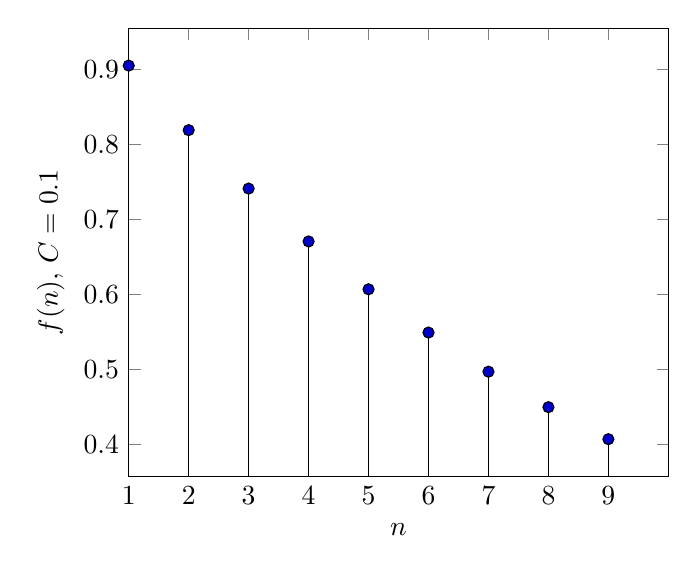
\begin{tikzpicture}
              \begin{axis}
                [
                  xlabel={$n$},
                  ylabel={$f(n)$, $C=0.1$},
                  xmin=1, xmax=10,
                  xtick={1,...,9}
                ]
                \addplot+[ycomb, domain=1:10, samples at={1,2,...,9}, black]{e^(-0.1*x)};
              \end{axis}
            \end{tikzpicture}
            \begin{tikzpicture}
              \begin{axis}
                [
                  xlabel={$n$},
                  ylabel={$f(n)$, $C=1$},
                  xmin=1, xmax=10,
                  xtick={1,...,9}
                ]
                \addplot+[ycomb, domain=1:10, samples at={1,2,...,9}, black]{e^(-1*x)};

              \end{axis}
            \end{tikzpicture}
            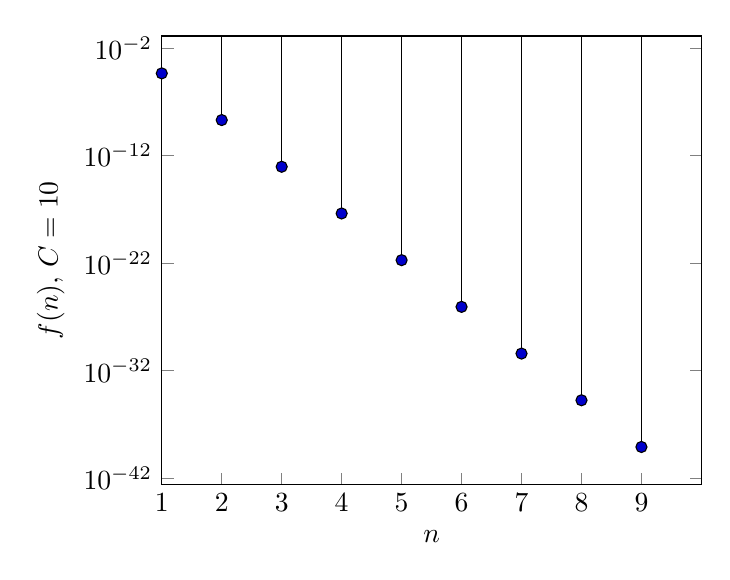
\begin{tikzpicture}
              \begin{axis}
                [
                  xlabel={$n$},
                  ylabel={$f(n)$, $C=10$},
                  ymode=log,
                  xmin=1, xmax=10,
                  xtick={1,...,9}
                ]
                \addplot+[ycomb, domain=1:10, samples at={1,2,...,9}, black]{e^(-10*x)};
              \end{axis}
            \end{tikzpicture}
          \end{center}
    \item Using the geometric series identity we proved in (a),
          $$S_{10}=\sum_{n=1}^{\infty}e^{-10n}=\sum_{n=1}^{\infty}(e^{-10})^n=\frac{1}{1-e^{-10}}\approx 1.00004540199,$$
          which is perfectly fine since $e^{-10}\ll 1$.
          Then
          $$I_{10}=\int_0^\infty e^{-10x}dx=-\frac{1}{10}\left[e^{-\infty}-e^{0}\right]=\frac{1}{10}$$
    \item Again using the geometric series identity since $e^{-0.1}< 1$, $S_{0.1}=1/(1-e^{-0.1})\approx 10.5$ and
          $$I_{0.1}=-\frac{1}{0.1}\left[e^{-\infty}-e^{0}\right]=10.$$
    \item This displays what we saw in class, the step size (in both cases above, $\Delta x=1$) is too big compared to the length scales over which
          $e^{-10n}$ is changing providing a poor approximation, but is fine over the scale of $e^{-0.1n}$ and provides a good approximation.
  \end{enumerate}
\end{soln}
\end{document}